\def\thecourse{18.466}
\def\thestudent{Zhilei Xu (929552018)}
\def\theprob{Midterm 2}
\documentclass[11pt]{article}
\usepackage{amsmath, graphicx, amsfonts}
\usepackage{fancyhdr}
\usepackage{lastpage}
\pagestyle{fancy}
\fancyhf{}
\fancyhf[HLEO]{\thestudent{}}
\fancyhf[HCEO]{\thecourse{} - Problem Set \theprob{}}
\fancyhf[HREO]{Page \thepage\ of \pageref{LastPage}}
\renewcommand\headrulewidth{0.4pt}
\newcommand{\argmax}{\mathrm{argmax}}
\newcommand\erf{\mathrm{erf}}
\newcommand\sgn{\mathrm{sgn}}
\newcommand{\widesim}[2][1.5]{
  \mathrel{\overset{#2}{\scalebox{#1}[1]{$\sim$}}}
}
\newcommand\eqnlabel[1]{\label{eqn:#1}}
\newcommand\eqnref[1]{(\ref{eqn:#1})}
\newcommand{\Beta}{\mathcal{B}}
\newcommand{\ProbS}{\iftrue}
\newcommand{\ProbE}{\fi}

\usepackage{titlesec, pgfplots, subcaption}
\titleformat{\section}[runin]{\Large\bfseries}{}{}{}
\titleformat{\subsection}[runin]{\normalfont\large\bfseries}{}{}{}
\begin{document}
\section*{1}
\subsection*{(a)}
$
\mu= E[X_i] = \frac{N+1}{2}
$,
so
$
\hat{N}_{MOM} =
2\bar{X}-1 = \frac{2}{3}(X_1+X_2+X_3)-1
$

\subsection*{(b)}
$
f(x | N) = \frac{I[x \leq N]}{N}, x=1,2,\dots
$,
so
$
f(X; N) = 
\frac{\prod_{i=1}^{3}I[X_i \leq N]}{N^3}
$,
hence
$
\hat{N}_{MLE} =
m = \max\{X_1, X_2, X_3\}
$

\subsection*{(c)}
$
Var[X_1] =
\left(\sum_{i=1}^{N} \frac{i^2}{N}\right) - \left(\frac{N+1}{2}\right)^2 =
\frac{(N+1)(2N+1)}{6} - \frac{(N+1)^2}{4} =
\frac{N^2-1}{12},
E[\hat{N}_{MOM}] =
E[2\bar{X}-1] = N
$, so
$
R(\hat{N}_{MOM},N) =
Var[\hat{N}_{MOM}] =
4Var[\bar{X}] =
\frac{4}{3} Var[X_1] = \frac{N^2-1}{9}
$.
\\
$
P_m(x) = P[m \leq x] = \prod_{i=1}^{3}P[X_i \leq x] =
\left(\frac{x}{N}\right)^3,
P[m = x] = \Delta P_m(x) =
\left(\frac{x}{N}\right)^3 -
\left(\frac{x-1}{N}\right)^3 =
\frac{3x^2-3x+1}{N^3}
$, \\
$
E[\hat{N}_{MLE}]=
\sum_{x=1}^{N} x\Delta P_m(x) =
[xP_m(x)] |_{0}^{N} - \sum_{x=1}^{N} P_m(x-1) \Delta x =
N P_m(N) - \sum_{x=1}^{N} P_m(x-1) =
$\\
$
N - \left(\sum_{x=1}^{N} (x-1)^3\right)/N^3 =
N - \left(\frac{N(N-1)}{2}\right)^2/N^3 =
\frac{(3N-1)(N+1)}{4N},
bias[\hat{N}_{MLE}] = \frac{-(N-1)^2}{4N}
$,\\
$
E[\hat{N}_{MLE}^2]=
\sum_{x=1}^{N} x^2\Delta P_m(x) =
\frac{\sum_{x=1}^{N} 3x^4 - 3x^3 + x^2}{N^3} =
\frac{(N+1)(36N^3+ 9N^2 - 19N + 4)}{60N^2},
Var[\hat{N}_{MLE}]=
\frac{(N^2-1)(9N^2-1)}{240N^2}
$ \\
$
R(\hat{N}_{MLE}, N) =
\frac{(N-1)^4}{16N^2} + 
\frac{(N^2-1)(9N^2-1)}{240N^2} =
%\frac{(N-1) ( 24N^3 - 36N^2 + 44N - 16 )}{240N^2}
%\frac{(N-1) ( 6N^3 - 9N^2 + 11N - 4 )}{60N^2}
\frac{(N-1) (2N-1) (3N^2-3N+4)}{60N^2}
$. Another direct way to compute: \\
Let
$
D = \hat{N}_{MLE}-N = m-N
$,
then
$
P[D=x] = P[m = x+N] =
\frac{3x^2 + (6N-3)x + (3N^2 - 3N + 1)}{N^3}
, 1-N \leq x \leq 0
$.\\
$
R(\hat{N}_{MLE}, N) =
E_N[D^2] =
\sum_{x=1-N}^{0} \frac{x^2[3x^2 + (6N-3)x + (3N^2 - 3N + 1)]}{N^3} =
\frac{(N-1)(2N-1)(3N^2 - 3N + 4)}{60N^2}
$. \\
Let
$
d(N) = {R(\hat{N}_{MOM}, N)} - {R(\hat{N}_{MLE}, N)} =
%\frac{60(N^2-1)N^2}{9(N-1)(2N-1)(3N^2-3N+4)} =
%\frac{N-1}{180N^2}\left[20N^2(N+1)-3(2N-1)(3N^2-3N+4)\right]
%\frac{N-1}{180N^2}\left[20N^3+20N^2-3(6N^3-3N^2 - 6N^2+3N + 8N-4)\right]
%\frac{N-1}{180N^2}\left[20N^3+20N^2-3(6N^3-9N^2 + 11N -4)\right]
%\frac{N-1}{180N^2}\left[20N^3+20N^2 -18N^3 +27N^2 -33N +12\right]
\frac{N-1}{180N^2}(2N^3+47N^2 -33N +12) =
\frac{N-1}{180N^2}f(N)
$,\\
$
f(1) = 28 >0,
\forall N \geq 1, f'(N) = 6N^2+94N-33 > 0
$, so
$
\forall N \geq 1, f(N)>0
$, \\
so we can see that
$
d(1) = 0
$
and
$
\forall N > 1, d(N) > 0
$. \\
So
$
\hat{N}_{MLE}
$
dominates
$
\hat{N}_{MOM}
$, 
and only when $N=1$, these two estimators have the same risk.

\iffalse
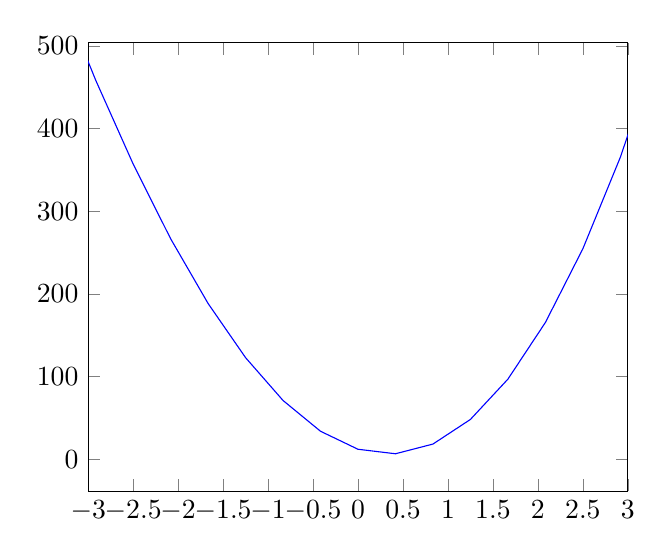
\begin{tikzpicture}
  \begin{axis}[
    xmin = -3,
    xmax = 3,
    xtick = {-3.0, -2.5, ..., 2.5, 3.0}
  ] 
  \addplot +[mark=none] {2*x^3+47*x^2-33*x+12}
  ;

  \end{axis}
\end{tikzpicture}
\fi

\subsection*{(d)}
The method of moment estimator can be improved by using the Rao-Blackwell theorem.\\
$
f(X; N) = 
\frac{\prod_{i=1}^{3}I[X_i \leq N]}{N^3} =
\frac{I[\max\{X_1, X_2, X_3\} \leq N]}{N^3}
$, so
$
m = \max\{X_1, X_2, X_3\}
$
is a sufficient statistic. \\
$
\hat{N}_{MOM} = 2\bar{X}-1 = \frac{2}{3}S-1
$, where
$ S=X_1+X_2+X_3$. \\
$
E[S | m] =
\sum_{i=1}^{m} P[X_1=i | m] \cdot E[S | m, X_1=i] =
$ \\
$
P[X_1=m | m] \cdot E[S | m, X_1=m] + \sum_{i=1}^{m-1} P[X_1=i | m] \cdot E[S | m, X_1=i] =
$ \\
$
\frac{m^2}{3m^2-3m+1}(m+E[X_2+X_3 | X_2 \leq m, X_3 \leq m]) + \sum_{i=1}^{m-1}\frac{2m-1}{3m^2-3m+1} \left(i+
E[X_2+X_3 | \max\{X_2, X_3\}=m]\right) =
$ \\
$
\frac{m^2(2m+1)}{3m^2-3m+1} + \frac{m(m-1)(2m-1)}{2(3m^2-3m+1)} +
\frac{(m-1)(2m-1)}{3m^2-3m+1}E[X_2+X_3 | \max\{X_2, X_3\}=m]
$

$
E[X_2+X_3 | \max\{X_2, X_3\}=m] =
$ \\
$
P[X_2 = m | \max\{X_2, X_3\}=m] \cdot (m+E[X_3 | X_3 \leq m]) +
\sum_{j=1}^{m-1}P[X_2 = j | \max\{X_2, X_3\}=m] \cdot (j+m) =
$ \\
$
\frac{m}{2m-1}(m+\frac{m+1}{2}) +
\frac{1}{2m-1} \cdot \frac{3m(m-1)}{2} =
\frac{3m^2-m}{2m-1}
$

So
$
E[S | m] =
\frac{m^2(2m+1)}{3m^2-3m+1} + \frac{m(m-1)(2m-1)}{2(3m^2-3m+1)} +
\frac{(m-1)(3m^2-m)}{3m^2-3m+1} =
\frac{3(2m^3-\frac{3m^2}{2}+\frac{m}{2})}{3m^2-3m+1}
$,\\
and the improved estimator
$
\hat{N}_{RB} = E[\frac{2}{3}S-1 | m] =
\frac{4m^3-3m^2+m}{3m^2-3m+1}-1 =
\frac{4m^3-6m^2+4m-1}{3m^2-3m+1} =
\frac{m^4-(m-1)^4}{m^3-(m-1)^3}
$ \\
$
E[\hat{N}_{RB}] =
\sum_{m=1}^{N} 
\frac{m^4-(m-1)^4}{3m^2-3m+1}
\cdot \frac{3m^2-3m+1}{N^3}
= N
$, so $\hat{N}_{RB}$ is unbiased. \\
$
E[\hat{N}_{RB}^2] =
\sum_{m=1}^{N} 
\frac{(m^4-(m-1)^4)^2}{(3m^2-3m+1)^2}
\cdot \frac{3m^2-3m+1}{N^3} =
\frac{1}{N^3}\sum_{m=1}^{N} 
\frac{(2m-1)^2(2m^2-2m+1)^2}{\frac{3}{4}(4m^2-4m+\frac{4}{3})} <
\frac{1}{N^3}\sum_{m=1}^{N} 
\frac{(2m-1)^2(2m^2-2m+1)^2}{\frac{3}{4}(4m^2-4m+1)} =
\frac{4}{3N^3}\sum_{m=1}^{N}(2m^2-2m+1)^2 =
\frac{4}{3N^3}\sum_{m=1}^{N}(4m^4-8m^3+8m^2-4m+1) =
\frac{4(4N^4+1)}{15N^2}
$, \\
$
R(\hat{N}_{RB}, N) = Var[\hat{N}_{RB}] <
\frac{4(4N^4+1)}{15N^2} - N^2 = \frac{N^4+4}{15N^2}
$. \\
For sufficiently large $N$ (such as $N \geq 3$),
$R(\hat{N}_{RB}, N)$ is close to $\frac{N^2}{15}$,
while $R(\hat{N}_{MOM}, N)$ is close to $\frac{N^2}{9}$,
so we can see that the method of moment estimator can be improved by using the Rao-Blackwell theorem.
For larger $N$, $R(\hat{N}_{MLE}, N)$ is close to $\frac{N^2}{10}$, so we can see that $\hat{N}_{RB}$ is even better than the maximum likelihood estimator for larger $N$.

\section*{2}
\subsection*{(a)}
Figures \ref{fig:linex}(\subref{fig:linex:0.2} - \subref{fig:linex:1}) are the plots for $l(\theta,a)$ as a function of $a-\theta$.
\begin{figure}[ht]
\centering
\foreach \c in {0.2, 0.5, 1} {
\subcaptionbox{c=\c \label{fig:linex:\c}}{
\begin{tikzpicture}
  \begin{axis}[
    xlabel={$a-\theta$},
    %ylabel={$l(\theta, a), c=\c$},
    xmin = -4.5,
    xmax = 3.5,
    xtick = {-4, ..., 3},
    width = 0.333\textwidth,
    height = 0.4\textwidth
  ] 
  \addplot +[mark=none] {e^(\c * x) - \c*x -1}
  %[yshift=8pt]
  %  node[pos=0.5] {$e^{\c(a-\theta)}-\c(a-\theta)-1$}
  ;
 
  \end{axis}
\end{tikzpicture}
}
}
\caption{plots for $l(\theta, a) = e^{c(a-\theta)}-c(a-\theta)-1$ as a function of $a-\theta$}
\label{fig:linex}
\end{figure}


\end{document}
